\section{Diverse}

  {\bf Bias:} When a user are able to make their own password, the password that is created is often influenced by different biases.  When we are talking about a bias in terms of passwords, a the password making process can be influenced by biases like the demography of a person or the visualization of the password scheme. 
    
  {\bf Mobile Devices: } When talking about graphical password, they are not widely adopted on mobile devices. There are still some graphical passwords that are made for mobile devices, and this section will give a state-of-the art on graphical passwords for mobile devices.
  Our mobile devices are used for different authentication task. In the background theory, it was stated that we had mainly three different authentication schemes, e.g. ``something you know'', ``something you have'', and ``something you are''.
  As stated earlier, 

  {\bf Password habits in subpopulations:} Password habits may be different across different subpopulation in cause of different background or culture. In 2012 Joseph Bonneau released a analysis of 70 million passwords from Yahoo! \cite{Bonneau2}. The data is analyzed in terms of guessing rate by using a dictionary attack. The collected data contained 328 subpopulations. The results showed that there was no ``good'' populations among the collected data, but there was a variation in the population. Demographically, the gender had a small effect in the guessing rate, but it showed that age tended to give effect where password strength increases across different age groups. The analysis also showed that language had a significantly effect on the password strength where Indonesian-speaking users were among the weakest subpopulations, and in contrast the German and Korean-speaking users provided relatively stronger passwords. 

  {\bf Passwords in a business setting:} Passwords are not just used in our private life, but also a requirement in a critical concern from a business point of view where the use of authentication for corporate systems, mobile, and room codes plays a major role in normal day of work. In corporate systems users are often promt with the a notification forcing them to change the password in a specified time interval. The problem with this is that user already have problems remembering their passwords as is. A research group conducted a questionnaire survey in a large organization \cite{habits2}. The goal was to get a understanding of password habits in a business point of view. The results showed that the users were prompt with password change 7 times a year causing 68\% of the employees to re-use the same password with a minor change in order to still be able to remembering their passwords.

  Since the first graphical password schemes was proposed, it is not widely in use. One of the problems with graphical approaches are that they require more overhead in the authentication phase. Like text-based passwords the users can simply type their passwords, while many of the graphical passwords require to go through many steps, requiring the user to spend more time in the authentication phase. The graphical password schemes like Passface and grIDsure are some of the graphical password schemes with commercial interest, while on mobile devices graphical passwords are not widely adopted. There is a known problem with authentication on mobile devices because of the difficulty of typing on mobile keyboards, making authentication schemes using alternatives getting increased attention. Because of the difficulty of writing on mobile keyboards it highlights the importance of understanding the usability and security implications.

%.----------------------------------------------------------------------------------

\chapter{Litterature Study}
  \section{Planning}
    This section will give a detailed plan for the structured litterature review, as well as building a 
    evaluation protocol for the review. 
    Research should be conducted in order to answer questions that have not been answerd yet. 
    By conducting a structured literature review, I can support my motivation for doing the research, 
    as well as get to know relevant research. 

    \section{Field of Study}
    Before conducting the litterature study, I will do a specification of my field of study in order to
    avoid a unsustainable broad scope. Too broas scope in a litterature study can give to irrelevant searches 
    and it will be hard to find the relevant information needed to answer the research questions. 

    In the figure below I have done a analysis of my field of study. The research will focus on authentication on mobile devices. 
    The type of authentication is screen locks. Finally the inner circle, the most specific topic, is the Android Unlock Pattern. 

    \begin{figure}[H]
    \centering
    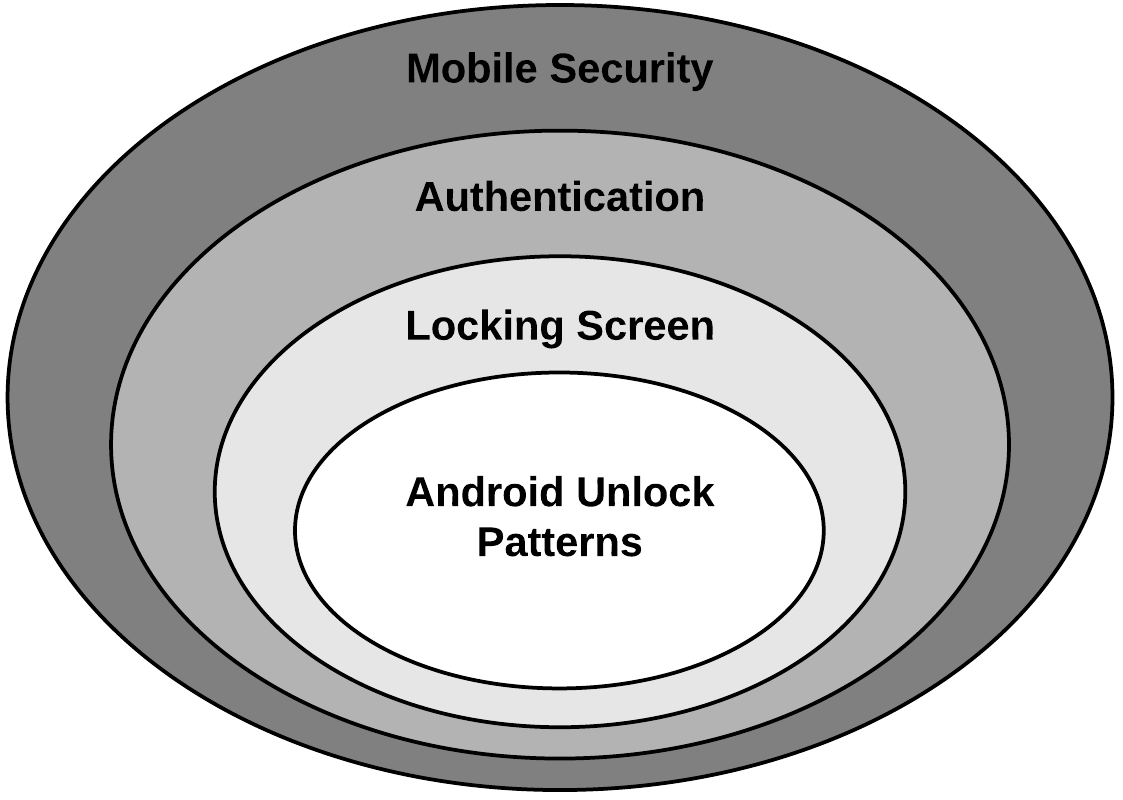
\includegraphics[scale=0.25]{pics/Fieldofstudy.png}
    \caption{Field of study}
    \end{figure}

    \section*{Keywords}  
    In the `field of study' I specified a specific scope in order to avoid to broad search space. 
    Inside each of the circles we can get more into details and create specific keywords that I will use in 
     the litterature search. 

    \begin{tabular}{ || l | l ||}
      \hline
      {\bf Mobile Security} & \\
      {\bf Locking Screen} &  \\
      {\bf Authentication} &  \\
      {\bf Android Unlock Patterns} & \\ 
      {\bf Psycology} & \\
      {\bf Graphical passwords} & \\
      \hline
    \end{tabular}
    \section*{Review Protocol}
